% Drawing 154/02-16 -- folder 154, batch 02, archive page 39 (PDF page 40).
% Transcription: figure : un disque au bord vert, traversé de cordes orange, deux faisceaux de cordes se croisant ; autour du bord, quatre arcs fléchés numérotés $1$, $2$, $3$, $4$ au crayon
% Kind: chord system in a disk with arrowed boundary arcs. Method 2 (redrawn from the facsimile). Status: ok.
% Notes: A disk with a (yellow-)green rim crossed by five orange chords, redrawn strand by strand from the 400 dpi facsimile (positions read off the colour mask): three nearly vertical chords from the top to the bottom of the rim, not crossing one another, and two chords sharing both their ends on the rim (upper right and lower left), forming a lens that each vertical chord crosses twice (once each chord); the shared ends are computed once on the rim. Around the rim the pencil arrows, two from each of the numbers 1, 2, 3, 4, going both ways along the rim. The pencil « (s, t) » above the disk belongs to the text of the page (the note on rubric a) and is not drawn. Redrawn 2026-11-09 (issue 128): to check again.
% Coordinates: 1 unit = 1 mm = 1/100 of the crop width (bbox in page fractions: [0.588, 0.127, 0.714, 0.217]).
% Redrawn by Claude (claude-opus-5-5), issue #73, 2026-11-07; not checked by a human; not compiled (no TeX in the session).
% Redrawn by Claude (claude-opus-5-5) 2026-11-09 (issue #128, third pass): strands traced one by one on the 400 dpi facsimile (positions read off the colour mask), pairwise crossings checked inside the disk, shared ends computed once, regions bounded by their strands; labels at \small. Not compiled. Status: ok.
% Rights: reproduces part of the work -- behind RENDER_TRANSCRIPTS, never published by itself.
\documentclass[tikz,border=3pt]{standalone}
\usepackage{amsmath,amssymb}
\usetikzlibrary{patterns,arrows.meta}
\tikzset{Or/.style={orange!90!black}, Ye/.style={yellow!80!orange}, Lg/.style={green!60!black!70}, Dg/.style={green!45!black}, Br/.style={brown!80!black}, Rd/.style={red!85!black}, Bl/.style={blue!70!black}, Gy/.style={black!40}, pencil/.style={black!45}, struck/.style={black!35}, mark/.style={circle,draw,inner sep=1.3pt}, pt/.style={circle,fill,inner sep=0.9pt}, opt/.style={circle,draw,fill=white,inner sep=1.1pt}}
\begin{document}
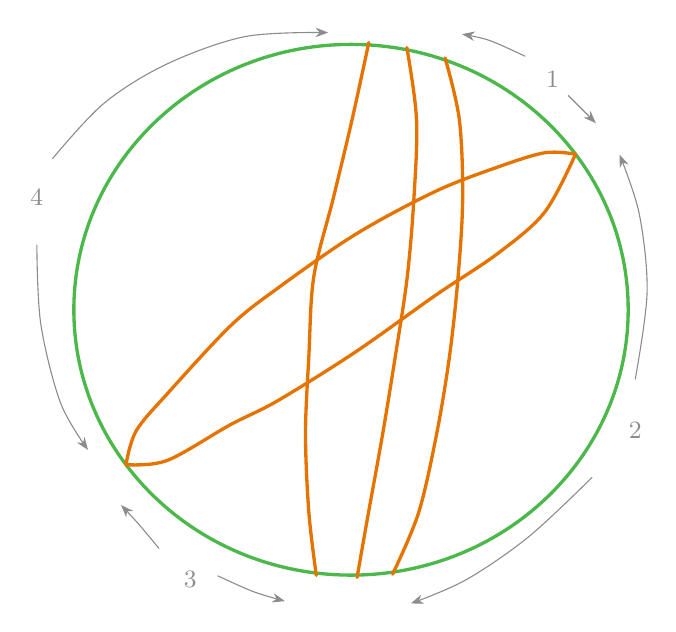
\begin{tikzpicture}[x=1mm,y=1mm,line cap=round,line join=round,font=\scriptsize]
\draw[Lg,very thick] (45.4,-54.2) ellipse[x radius=35.2, y radius=33.7];
\draw[Or,very thick] plot[smooth, tension=0.55] coordinates {(73.91,-34.44) (70.01,-34.26) (64.03,-36.08) (56.09,-39.18) (45.96,-44.63) (36.11,-51.45) (30.12,-56.22) (22.12,-64.81) (18.11,-69.59) (16.82,-73.87)};
\draw[Or,very thick] plot[smooth, tension=0.55] coordinates {(73.91,-34.44) (70,-41.8) (64.04,-47.05) (56.12,-52.37) (45.97,-59.56) (36.09,-65.75) (30.06,-68.81) (22.05,-73.34) (16.82,-73.87)};
\draw[Or,very thick] plot[smooth, tension=0.55] coordinates {(47.66,-20.27) (45.54,-30.03) (43.15,-40.03) (40.68,-49.95) (40.05,-60.01) (39.62,-70) (40.05,-79.99) (40.99,-87.93)};
\draw[Or,very thick] plot[smooth, tension=0.55] coordinates {(52.49,-20.9) (53.72,-29.99) (53.39,-40.02) (52.54,-50.04) (51.04,-60.04) (49.41,-70.03) (47.61,-80.02) (46.17,-88.19)};
\draw[Or,very thick] plot[smooth, tension=0.55] coordinates {(57.35,-22.23) (59.15,-29.99) (59.58,-40) (59,-50) (57.92,-60.02) (56.26,-70.05) (53.96,-80.05) (50.68,-87.78)};
\draw[pencil,-{Stealth[length=1.6mm]}] plot[smooth, tension=0.55] coordinates {(7.5,-35) (14,-28) (22,-23) (32,-19.5) (42.5,-19)};
\draw[pencil,-{Stealth[length=1.6mm]}] plot[smooth, tension=0.55] coordinates {(5.5,-46) (6,-56) (8.5,-66) (12,-72)};
\draw[pencil,-{Stealth[length=1.6mm]}] plot[smooth, tension=0.55] coordinates {(21,-84.5) (18.5,-81.5) (16.2,-79)};
\draw[pencil,-{Stealth[length=1.6mm]}] plot[smooth, tension=0.55] coordinates {(28.5,-88) (33,-90) (37,-91.2)};
\draw[pencil,-{Stealth[length=1.6mm]}] plot[smooth, tension=0.55] coordinates {(76,-75.5) (68,-83) (60,-88.5) (53,-91.5)};
\draw[pencil,-{Stealth[length=1.6mm]}] plot[smooth, tension=0.55] coordinates {(81.5,-63) (83,-52) (82,-42) (79.5,-34.5)};
\draw[pencil,-{Stealth[length=1.6mm]}] plot[smooth, tension=0.55] coordinates {(73,-27) (76.5,-30.5)};
\draw[pencil,-{Stealth[length=1.6mm]}] plot[smooth, tension=0.55] coordinates {(67.5,-22) (63,-20) (59.5,-19.2)};
\node[inner sep=1pt,pencil] at (71,-25) {\small $1$};
\node[inner sep=1pt,pencil] at (81.5,-69.5) {\small $2$};
\node[inner sep=1pt,pencil] at (25,-88.5) {\small $3$};
\node[inner sep=1pt,pencil] at (5.5,-40) {\small $4$};
\end{tikzpicture}
\end{document}
